%%%%%%%%%%%%%%%%%%%%%%%%%%%%%%%%%%%%%%%%%%%%%%%%%%%%%%%%%%%%%%%%%%%%%%%%%%%%%%%%%%%%%%%%%%%%%%%%%%%
\begin{frame}
	\frametitle{Shor}
		\framesubtitle{Overview}
		\begin{enumerate}
		\item[1.]{Pick a random number $a < N$ and compute $gcd(a, N)$.}\\
		\item[2.]{If $gcd(a, N) \neq 1$, then this number is a nontrivial factor of N, so we are done.}\\
		\item[3.]{Otherwise, use the period-finding subroutine (below) to find r, the period of the following function:}
		$$f(x)=a^{x}{\bmod {N}}$$
i.e. the order $r$ of $a$ in $(\mathbb {Z} _{N})^{\times }$ $(\mathbb {Z} _{N})^{\times }$, which is the smallest positive integer $r$ for which $f(x+r)=f(x)$, or $f(x+r)=a^{x+r}{\bmod {N}}\equiv a^{x}{\bmod {N}}$ 
		\item[4.]{If $r$ is odd, go back to step 1.}\\
		\item[5.]{If $a^{ \frac{r}{2}} \equiv -{1 \bmod{N}}$, go back to step 1.}\\
		\item[6.]{$gcd(a^{ \frac{r}{2}} + 1, N)$ and $gcd(a^{ \frac{r}{2}} - 1, N)$ are nontrivial factors of N.}\\
		\end{enumerate}
\end{frame}
%%%%%%%%%%%%%%%%%%%%%%%%%%%%%%%%%%%%%%%%%%%%%%%%%%%%%%%%%%%%%%%%%%%%%%%%%%%%%%%%%%%%%%%%%%%%%%%%%%%

%%%%%%%%%%%%%%%%%%%%%%%%%%%%%%%%%%%%%%%%%%%%%%%%%%%%%%%%%%%%%%%%%%%%%%%%%%%%%%%%%%%%%%%%%%%%%%%%%%%
\begin{frame}
	\frametitle{Fast exponentiation}
		\framesubtitle{}

		{\normalsize
		\hspace{0.5cm}{We can calculate $A^{B} \mod(C)$ quickly, using modular multiplication rules:
$$A ^{2} \mod(C) = (A \times A) \mod(C) = ((A\mod(C)) \times (A\mod(C))) \mod(C)$$}\\
		}
		

\end{frame}
%%%%%%%%%%%%%%%%%%%%%%%%%%%%%%%%%%%%%%%%%%%%%%%%%%%%%%%%%%%%%%%%%%%%%%%%%%%%%%%%%%%%%%%%%%%%%%%%%%%

%%%%%%%%%%%%%%%%%%%%%%%%%%%%%%%%%%%%%%%%%%%%%%%%%%%%%%%%%%%%%%%%%%%%%%%%%%%%%%%%%%%%%%%%%%%%%%%%%%%
\begin{frame}
	\frametitle{Shor}
		\framesubtitle{Scheme}
	\vspace{0.5cm}
		\begin{figure}
		\centering
			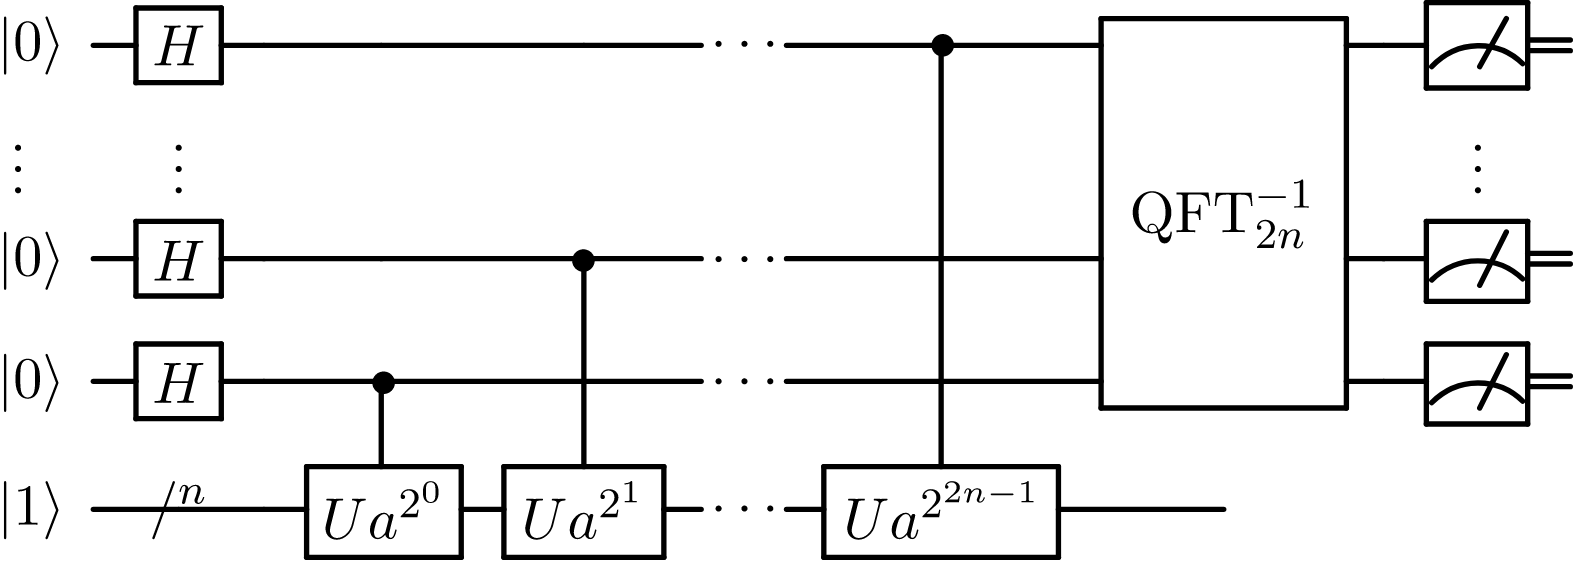
\includegraphics[scale=0.25]{shor}
			\label{fig:shor shor}
		\end{figure}

\end{frame}
%%%%%%%%%%%%%%%%%%%%%%%%%%%%%%%%%%%%%%%%%%%%%%%%%%%%%%%%%%%%%%%%%%%%%%%%%%%%%%%%%%%%%%%%%%%%%%%%%%


%%%%%%%%%%%%%%%%%%%%%%%%%%%%%%%%%%%%%%%%%%%%%%%%%%%%%%%%%%%%%%%%%%%%%%%%%%%%%%%%%%%%%%%%%%%%%%%%%%%
\begin{frame}
	\frametitle{Quantum Fourier transform}
		\framesubtitle{}

		\begin{figure}
		\centering
			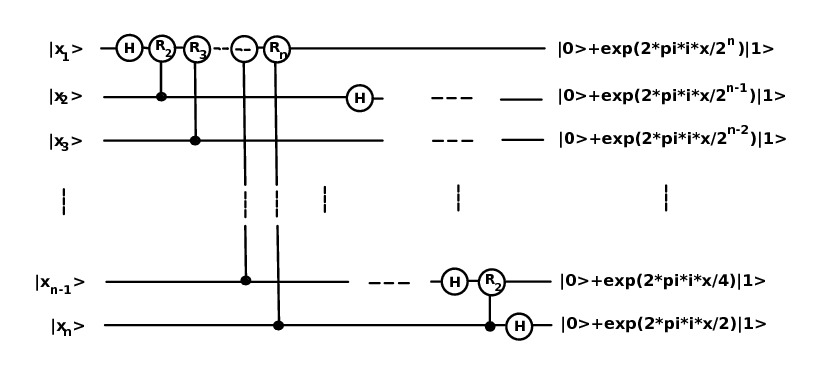
\includegraphics[scale=0.4]{qftsimple}
			\label{fig:qft qft}
		\end{figure}
		

\end{frame}
%%%%%%%%%%%%%%%%%%%%%%%%%%%%%%%%%%%%%%%%%%%%%%%%%%%%%%%%%%%%%%%%%%%%%%%%%%%%%%%%%%%%%%%%%%%%%%%%%%%